\documentclass[fleqn]{article}
\usepackage{graphicx} 
\usepackage{here}    
\usepackage{amsmath}
\textwidth=15.0cm
\textheight=22.0cm
\topmargin=-1cm
\oddsidemargin=-0.3cm
\evensidemargin=-0.3cm


%packages
\usepackage{amsmath}
\usepackage{cite}
\usepackage[toc,page]{appendix}
\usepackage{fancyvrb}
\usepackage{tikz}
\usepackage{multicol}
\usepackage{framed}
\usepackage{pgfplots}
\usepackage{fixltx2e}
\usepackage{subfigure}
\usepackage{lscape}
\usepackage{enumitem}
\usepackage{multirow}
\usepackage{color}
\usepackage{xcolor}
\usepackage{comment}
\usepackage{changes}
\renewcommand*\descriptionlabel[1]{\hspace\leftmargin$#1$}

%tikz labraries
\usetikzlibrary{matrix}
\usetikzlibrary{decorations.pathreplacing}
\usetikzlibrary{positioning}
\usetikzlibrary{calc}
\usetikzlibrary{shapes,arrows, chains}
\usetikzlibrary{intersections}
\usetikzlibrary{decorations.markings}
\usetikzlibrary{calc,intersections}
\usetikzlibrary{patterns}


\makeatletter
\def\mathcolor#1#{\@mathcolor{#1}}
\def\@mathcolor#1#2#3{%
  \protect\leavevmode
  \begingroup
    \color#1{#2}#3%
  \endgroup
}
\makeatother

%##### DEFINE YOUR NAME #########################
\definechangesauthor[color=blue,name={Arpad Rozsas}]{AR}
\definechangesauthor[color=red,name={Nadieh Meinen}]{NEM}
%###########################################

\begin{document}


\section{Review of existing literature} 
 

\subsection{Davenport Wind Loading Chain}
\added[id=NEM]{Some history regarding the development of the DWLC may be added here}\\
Due to its conceptual ease, the DWLC is the foundation of many wind load models found in current codes of practice \cite{Davenport_2002}. The DWLC provides a conceptual representation of the synthesis of extreme wind loads and is thought of as a 'chain' consisting on a number of 'links' each representing a relevant physical aspect contributing to the wind load. \\
\\
The first link of the chain, "wind climate", accounts for the characteristics of the large-scale wether systems which depend on the geographical location of the building. The wind climate is represented by a time-averaged wind speed corresponding to a standard exposure, averaging time and reference time. \\
\\
The second link of the chain, "terrain effects", corrects for the influences of the upwind terrain which cause the increase of mean wind speed with height and the terrain-introduced wind-gustiness. As the upwind terrain differs per incident wind direction, also the "terrain effects" differ per incident wind direction.  \\
\\
The third link of the chain "aerodynamic effects" accounts for the (local) increase in wind speed due to the aerodynamic shape of the building, as well as the wind gusts introduced by local vortex shedding at the edges of the building. Besides, it takes into account the effects of a non-uniform pressure distribution over the reference area, resulting in relatively lower forces at larger tributal areas. Depending on the location on the building and incident wind direction, the aerodynamic effects result in either high compression forces (maxima) or high suctional forces (minima). \\
\\
The fourth link of the chain "dynamic effects" accounts for the potential wind-induced resonant vibrations, which depend on the damping ratio and natural frequency of the building.  
In case of dynamic insensitive structures or structural, the wind-induced resonant vibrations are negliglible. \\
\\
The fifth link of the chain, "criteria", recognizes that clear crtieria must be in place for judging the acceptability of the predicted loads and responses for both ultimate limit states and serviceability limit states. 


\begin{figure}[H]
\label{fig:wind_loading_chain}
\centering
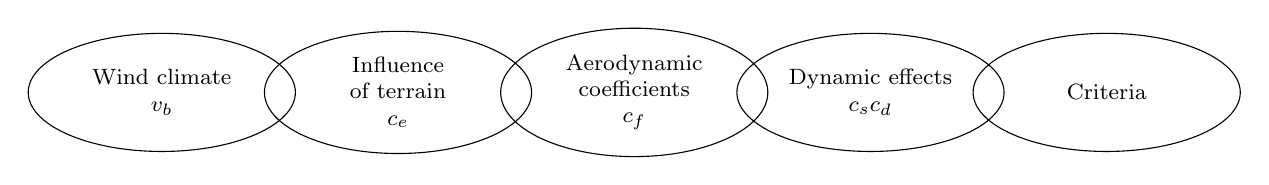
\begin{tikzpicture}[node distance = 3 cm, auto]
% tikz settings
\footnotesize
\tikzstyle{block} = [ellipse, draw,  
    text width=2.2cm, text centered,  rounded corners ,minimum height=1.5cm]
\tikzstyle{line} = [draw, latex-latex]

% the tikz picture
\node [block, align=center] (windclimate) {Wind climate \\ $v_b$};
\node [block, align=center, right of=windclimate] (influenceofterrain) {Influence of terrain \\ $c_e$ };
\node [block, align=center, right of=influenceofterrain] (Aerodynamic) {Aerodynamic coefficients \\ $c_f$};
\node [block, align= center, right of=Aerodynamic] (Dynamic) {Dynamic effects \\ $c_sc_d$};
\node [block, align=center, right of=Dynamic] (criteria) {Criteria};
\end{tikzpicture}
\caption{Davenport Wind Loading Chain, based on  \cite{Davenport_2002}}
\end{figure}

\noindent
For a propor representation of the structural reliability, the uncertainties in each of the links in the DWLC as well as the effects of wind-directionality need to be discounted for in the reliability analysis \cite{Davenport_1983b}. However, both the probabilistic modeling of the individual links in the chain, as well as methods to deal with wind-directionality effects, are still under active debates in the scientific cummunity. Besides, only a limited number of research exists that provides a full-probabilistic assessment of wind-loaded structural elements. \\
\\
In the following sections, an overview is presented of the most important findings regarding the probabilistic modeling of the individual links in the DWLC (see SECTION), the probabilistic methods for taking into account wind directionality effects (see SECTION) and the published results regarding full-reliability calculations (see SECTION). In section SECTION a motivation of out modeling choices is presented.



\subsection{Probabilistic modeling of of DWLC components}
Most of these discussions are related to the probabilistic modeling of the 'wind climate' and the 'aerodynamic coefficients', whilst little attention is directed towards the probabilistic modeling of the 'influence of terrain'. The reason for this is twofold. First, the 'influence of terrain' is assumed to have a lesser contribution to the total wind load effect than the other two \cite{} and second, data regarding the 'influence of terrain' are scarse. Consequentially, the probabilistic modeling of the 'influence of terrain' generally occurs on the basis of the probabilistic model code \cite{PMC, Hansen_2015} or on the basis of expert knowledge \cite{Sedlacek}.\\
\\
Both the probabilistic modeling of the 'wind climate' and 'aerodynamic coefficients' regard the probabilistic modeling of extremes. 
The discussions in both links therefore have many similarities. The main points of discussion thereby are (1) the extremal analysis method and distribution type to be used for the modeling and (2) the parameter interference techniques to be applied for the distribution fitting. Both issues will be addressed below. 



\subsubsection{Extremal analysis method (and distribution type)}
The extreme wind speeds and the extreme pressure coefficients are generally modeled on the basis of measurement data in combination with extremal analysis methods. 
Literature provides a numerous amount of extremal analysis methods and distribution models for the probabilistic modeling of extremes. Roughly, these methods can be distinguished in block maxima methods (BM), and the Peak over Theshold methods, and extensions to these methods. In \cite{Palutikov} an overview is provided of applications of these methods on wind speeds. In \cite{} an overview is provided of applications of these methods on pressure coeficients. \\
\\
\textit{Block maxima methods}\\
The basis of the BM methods lies in the division of the observation period into nonoverlapping blocks (periods of equal size) and restricts attention to the maximum observation in each block, over which an extreme value distribution is fitted. The main assumptions of the BM method are independent and identically distributed (i.i.d) random variables and convergion of the parent distribution towards the Generalized Extreme Value distribution (GEV). \\
\\
Within wind engineering, discussions regarding  the BM method are related to (1) the minimum block-duration to ensure statistically independent extremes and (2) which extreme value distribution to fit on the extremes. 
\begin{itemize}
\item In the case of extreme wind speeds, the block-duration is gerenally chosen to be one year. The main reason for this is to capture seasonal effects, rather than to ensure statistically independency. A more pronounced discussion exists regarding the distribution type to fit on the extremes. Traditionally the Gumbel distribution is taken. The theoretical justification of this distribution lies in the widely accepted assumption that the parent wind speeds are distributed by the reversed two parameter Weibull distribution, of which the extremes converge towards the Gumbel distribution \cite{Cook,Gumbel?}. However, based on Pickands GPD model estimation\cite{} and domain of attraction discrimination \cite{} \cite{Lechner_1992} compared the results of 100 US-wind records and found that in 61 cases the Weibull (W2/3?) distribution was the best fit, 36 the Gumbel distribution and in 3 cases the Frechet distribution was the best fit. Gomez and Vickery state that, in cases of mixed climates, the Fr\'{e}chet distribution is the best.

\item In the case of the extreme pressure coefficients the minimum required block-duration is less of a settled issue. Cook and Mayne [1] based the minimum record-length on the lower limit of the Spectral Gap in the Macrometeorological spectrum and suggested that one record should have a minimum length of 10 minutes. Lou and Peterka [4] used signal autocorrelation as a measure of dependency between extremes and found that periods smaller than 1 minute would already suffice. A recent study \cite{Meinen_2015} showed that the sample duration could be shortened to 10 seconds. Comparisons of the effect of different block-durations on the level of the Cook-Maybe fractile may be found in the literature as well \cite{Cook}\cite{Gavanski_2013}\cite{Peng201411} \cite{Quan_2014} and found that the results were significant. \\
\\
The type of Extreme Value distribution that should be fitted on the extreme pressure coefficients is neither a settled issue. In most  cases the Gumbel distribution is fitted. Kasperski however \cite{Kasperski2003527} discusses the use of the upper-bounded Weibull distribution, for reasons that wind tunnels cannot produce unlimited pressures for a given mean wind speed. Based on a statistical analysis of measurement data, he finds that in most of the cases indeed the W2/3 distribution best fits the data and in some cases the Frechet or Gumbel distribution. Similar findings are made by other researchers \cite{Holmes2003893, Quan_2014}. 
\end{itemize}

\textit{POT method}\\
In the POT, one selects those of the initial observations that exceed a certain high threshold after which the
Pareto distribution is fitted \cite{Pickands_1975}. Main discussions are related to the height of the threshold value and the methods to ensure statistically independent extremes. 
\begin{itemize}
\item POT and extreme wind speeds?
\item POT and extreme pressure coefficients?
\end{itemize}

\subsubsection{Distribution parameter interference techniques}
\added[id=NEM]{By arpad}\\
Some papers addressing the importance of sampling errors on the design wind speeds:
\begin{itemize}
\item Simiu \textit{et. al} \cite{Simiu_1978} investigated (among others) the effects of sampling errors on the estimation of design wind speeds from a confindent interval approach and found them to be significant.
\item 
Rojiani and Wen \cite{Rojiani_1980} also (among others) investigated the effects of sampling uncertainties on the design wind speeds and found that the effects of distribution type and parameter esitmation technique were of larger signifance. 
\end{itemize}

\subsection{Wind directionality}
Several researchers have investigated the influence of wind-directionality on the design wind loads. \\
Simiu and Filiben \cite{Simiu_1981} show that "cladding loads calculated without taking directional information on extreme wind speeds into account may in certain cases be larger than the actual loads by a factor of two or more." \\
Isyumov \textit{et. al} \cite{Isyumov_2014} state that "the ASCE 7 directional factor of Kd=0.85 is not unreasonable for the structural and cladding loads for buildings located in areas, where extra-tropical winds dominate." \\
Davenport \cite{Davenport_1983b} estimated the differences in the risks in the design of cladding pressures when the influence of wind direction is taken into account and found that "if the peak pressure coefficient aligns with a direction of relatively weak winds, the reduction can easily be a factor two". 

\subsection{Full probabilistic analysis}
As stated before, the focus of the literature is mostly on the in-depth analysis of a single, selected link only. In the literature, a handful of studies may be found that provide a full-probabilistic assessment which accounts for the uncertainties in the entire DWLC.  \\
\\
The ones were Cook and Mayne \cite{Mayne1979109}, who developed a method \added[id=NEM]{often referred to as 'the Simplified Method'} to account for the uncertainties in the wind speeds and the pressure coefficients, where the uncertainties in the other links were kept deterministic.  Many researchers \cite{Kasperski2003527,Harris_2003} have used, discussed and refined this method.\\
\\
Some recent studies did account for the uncertainties in all links jointly. \\
E.g. for the purpose of partial factor calibration Hansen \cite{Hansen_2015} and Sedlacek provide a full probabilistic design method that takes into account uncertainties in all links. For the probabilistic modeling of each of the parameters choices were made based on literature / sample data. The effects or their modeling choices on the reliability level were however not investigated. \\
\\
In a super amazing pioneer study \added[id=NEM]{just kidding}, Meinen investigated the influence of some modeling choices ont he reliability level of an element. The results showed that.. ? It is actually interesting to look at the influence of modeling choices on beta-level, as it has a large impact. \\
\\
As a result, only limited knowledge exists on the effects of modeling choices on the structural reliability of wind-loaded structural elements, i.e. uncertainty propagation.



\subsection{Our choices with respect to the modeling of extremes}
As it it 

In this research the block-method combined with the Generalized Extreme Value distribution is adopted \cite{CUR_103} \cite{Kasperski2003527} \cite{Holmes2003893}. 





\end{document}

